\documentclass[11pt]{article}
\usepackage[utf8]{inputenc}
\usepackage[T1]{fontenc}
\usepackage{amsmath}
\usepackage{amssymb}
\usepackage{multicol}
\usepackage{geometry}
\usepackage{tikz}
\usepackage{enumitem}
\usepackage{xcolor}
\usepackage{titlesec}

% Configurações de layout
\geometry{a4paper, left=1cm, right=1cm, top=0.5cm, bottom=1.2cm}
\setlength{\columnseprule}{0.4pt}

% Cores para títulos
\titleformat{\section}{\normalfont\Large\bfseries\color{blue}}{\thesection}{1em}{}
\titleformat{\subsection}{\normalfont\large\bfseries\color{red}}{\thesubsection}{1em}{}

\title{\textcolor{red}{Primeiro Trimestre: Combinatória
    \\Princípio Fundamental da Contagem, Arranjo, Permutação e Combinação}}
\author{Professor: Jefferson}
\date{}

\begin{document}

\maketitle
\vspace{-1cm}

\begin{multicols}{2}

\section*{Conceitos Básicos}

\subsection*{Combinatória}
Ramo da matemática que estuda técnicas de contagem, permitindo contar o número de maneiras diferentes de organizar, selecionar ou arranjar objetos, sem necessidade de listar todas as possibilidades.

\subsection*{Princípio Fundamental da Contagem (PFC)}
Se um evento é composto por duas ou mais etapas sucessivas e independentes, o número total de formas diferentes de ocorrer é o produto das quantidades de possibilidades em cada etapa.

Se a primeira etapa pode ocorrer de $m$ formas e a segunda de $n$ formas:
\[
\text{Total} = m \times n
\]

\subsection*{Variáveis}
\begin{itemize}
\item $n$: número total de elementos
\item $p$: número de elementos a serem escolhidos ou arranjados
\item $P(n, p)$: arranjo de $n$ elementos tomados $p$ a $p$
\item $C(n, p)$: combinação de $n$ elementos tomados $p$ a $p$
\item $n!$: fatorial de $n$ (produto de todos os inteiros positivos até $n$)
\end{itemize}

\section*{Fatorial}

\subsection*{Definição}
O fatorial de um número natural $n$, denotado por $n!$, é o produto de todos os inteiros positivos de 1 até $n$.

\[
n! = n \times (n-1) \times (n-2) \times \ldots \times 2 \times 1
\]

Por definição: $0! = 1$

\subsection*{Exemplos}
\begin{itemize}
\item $3! = 3 \times 2 \times 1 = 6$
\item $4! = 4 \times 3 \times 2 \times 1 = 24$
\item $5! = 5 \times 4 \times 3 \times 2 \times 1 = 120$
\end{itemize}

\section*{Permutação}

\subsection*{Definição}
Permutação é um arranjo de todos os $n$ elementos de um conjunto, onde a ordem importa. É o número de maneiras diferentes de organizar $n$ objetos distintos.

\subsection*{Fórmula}
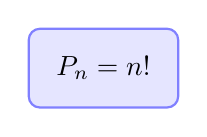
\begin{tikzpicture}
\node[rectangle, fill=blue!10, rounded corners, inner sep=10pt, draw=blue!50, thick] (box) {
$P_n = n!$
};
\end{tikzpicture}

\subsection*{Exemplo}
De quantas maneiras 3 pessoas podem se alinhar em uma fila?
\[
P_3 = 3! = 3 \times 2 \times 1 = 6
\]

\section*{Arranjo}

\subsection*{Definição}
Arranjo é a seleção de $p$ elementos de um conjunto de $n$ elementos, onde a ordem importa. Representa o número de maneiras de escolher e organizar $p$ objetos de um total de $n$ objetos.

\subsection*{Fórmula}
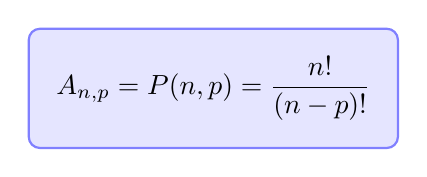
\begin{tikzpicture}
\node[rectangle, fill=blue!10, rounded corners, inner sep=10pt, draw=blue!50, thick] (box) {
$A_{n,p} = P(n,p) = \dfrac{n!}{(n-p)!}$
};
\end{tikzpicture}

\subsection*{Exemplo}
De quantas maneiras podemos escolher e organizar 2 pessoas de um grupo de 4 para as posições de presidente e vice-presidente?
\[
A_{4,2} = \frac{4!}{(4-2)!} = \frac{4!}{2!} = \frac{24}{2} = 12
\]

\section*{Combinação}

\subsection*{Definição}
Combinação é a seleção de $p$ elementos de um conjunto de $n$ elementos, onde a ordem NÃO importa. Representa o número de formas diferentes de escolher um subconjunto de $p$ objetos de um total de $n$ objetos.

\subsection*{Fórmula}
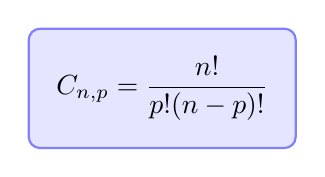
\begin{tikzpicture}
\node[rectangle, fill=blue!10, rounded corners, inner sep=10pt, draw=blue!50, thick] (box) {
$C_{n,p} = \dfrac{n!}{p!(n-p)!}$
};
\end{tikzpicture}

\subsection*{Exemplo}
De quantas maneiras podemos escolher 2 pessoas de um grupo de 4 para uma comissão (a ordem não importa)?
\[
C_{4,2} = \frac{4!}{2!(4-2)!} = \frac{24}{2 \times 2} = \frac{24}{4} = 6
\]

\section*{Diferença entre Arranjo e Combinação}

\subsection*{Quando usar Arranjo}
A ordem dos elementos importa. Exemplos:
\begin{itemize}
\item Escolher presidente, vice-presidente e secretário
\item Senhas e códigos
\item Primeiras, segundas e terceiras posições em uma corrida
\end{itemize}

\subsection*{Quando usar Combinação}
A ordem dos elementos não importa. Exemplos:
\begin{itemize}
\item Escolher membros de uma comissão
\item Seleção de frutas para um suco
\item Cartas de um baralho
\end{itemize}

\section*{Exercícios Básicos - Princípio Fundamental da Contagem}

\begin{enumerate}[leftmargin=*]

\item Uma loja vende camisetas em 5 cores e calças em 3 cores. Quantas combinações diferentes de roupa pode um cliente escolher?

\item Um restaurante oferece 4 entradas, 6 pratos principais e 3 sobremesas. De quantas maneiras diferentes um cliente pode fazer um pedido (1 entrada, 1 prato, 1 sobremesa)?

\item Quantas placas de carro podem ser formadas com 3 letras (sem repetição) seguidas de 4 números? Considere 26 letras.

\item Uma senha possui 3 dígitos. Quantas senhas diferentes existem se os dígitos podem se repetir?

\end{enumerate}

\section*{Exercícios Básicos - Permutação}

\begin{enumerate}[leftmargin=*, start=5]

\item Calcule:
\begin{enumerate}[label=\alph*)]
\item $3!$
\item $5!$
\item $6!$
\end{enumerate}

\item De quantas maneiras 4 pessoas podem se alinhar em uma fila?

\item Quantas maneiras diferentes existem para organizar as letras da palavra AMOR?

\item Quantas permutações possui um conjunto de 7 elementos?

\end{enumerate}

\section*{Exercícios Básicos - Arranjo}

\begin{enumerate}[leftmargin=*, start=9]

\item Calcule:
\begin{enumerate}[label=\alph*)]
\item $A_{5,2}$
\item $A_{8,3}$
\item $P(7,2)$
\end{enumerate}

\item De quantas maneiras 5 atletas podem ocupar as 3 primeiras posições de uma corrida?

\item Em uma corrida com 10 participantes, de quantas formas diferentes podemos escolher o 1º, 2º e 3º lugar?

\item Um código de segurança usa 4 dígitos diferentes. Quantos códigos podem ser formados com os 10 algarismos?

\end{enumerate}

\section*{Exercícios Básicos - Combinação}

\begin{enumerate}[leftmargin=*, start=12]

\item Calcule:
\begin{enumerate}[label=\alph*)]
\item $C_{6,2}$
\item $C_{10,3}$
\item $C_{8,4}$
\end{enumerate}

\item De quantas formas podemos escolher 3 alunos de uma turma de 10 para uma comissão?

\item De um grupo de 8 pessoas, quantas comissões de 4 pessoas podem ser formadas?

\item De quantas maneiras diferentes podemos escolher 2 frutas de um conjunto de 7 frutas diferentes?

\end{enumerate}

\end{multicols}

\end{document}
